\documentclass[dvipdfmx]{jsarticle}
\usepackage{tikz}
\usetikzlibrary{calc, quotes, angles}%quotesは角度のラベルオプション内に記述するために使用
\begin{document}
%直角記号の付け方の例1(calc ライブラリ必須)
\begin{tikzpicture}
 \draw
 (20:3cm) coordinate (A) node[right] {A}
 -- (0,0) coordinate (O) node[below left] {O}
 -- (110:2cm) coordinate (C) node[above left] {C};
 \coordinate (P) at ($(O)!.3cm!(A)!.3cm!90:(A)$);%直角記号の頂点の設定
 \draw[thick, red] ($(O)!(P)!(A)$)--(P);
 \draw[thick, red] ($(O)!(P)!(C)$)--(P);
\end{tikzpicture}
%直角記号の付け方の例2(calc ライブラリ必須)
\begin{tikzpicture}
 \draw
 (20:3cm) coordinate (A) node[right] {A}
 -- (0,0) coordinate (O) node[below left] {O}
 -- (110:2cm) coordinate (C) node[above left] {C};
 \draw[thick, red] ($(O)!8pt!(A)$)--($(O)!8pt!(A)!8pt!90:(A)$)--($(O)!8pt!(C)$);
\end{tikzpicture}
%一般の角度記号の付け方(3.0.0以降,angles ライブラリ必須)
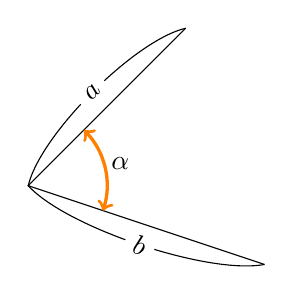
\begin{tikzpicture}
 \draw
 (3,-1) coordinate (A)
 -- (0,0) coordinate (B)
 -- (2,2) coordinate (C)
 pic["$\alpha$",draw=orange, <->, very thick, angle eccentricity=1.2, angle radius=1cm] {angle=A--B--C};
%線分の長さを示す例
 \draw (B).. controls ($(B)!.2!(C)!10pt!90:(C)$) and ($(B)!.8!(C)!10pt!90:(C)$) .. (C) node [midway, sloped, fill=white] {$a$};
 \draw (A).. controls ($(A)!.2!(B)!10pt!90:(B)$) and ($(A)!.8!(B)!10pt!90:(B)$) .. (B) node [midway, sloped, fill=white] {$b$};
\end{tikzpicture}


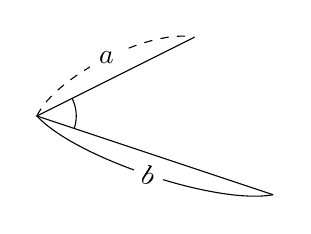
\begin{tikzpicture}
 \coordinate (A) at (3, -1) node at (A) {};
 \coordinate (B) at (0, 0) node at (B) {};
 \coordinate (C) at (2, 1) node at (C) {};

 %線分の長さを示す例
 \draw [dashed] (B).. controls ($(B)!.2!(C)!10pt!90:(C)$) and ($(B)!.8!(C)!10pt!90:(C)$) .. (C) node [midway,fill = white] {$a$};
 \draw (A).. controls ($(A)!.2!(B)!10pt!90:(B)$) and ($(A)!.8!(B)!10pt!90:(B)$) .. (B) node [midway, sloped, fill=white] {$b$};
 
 \draw
 (A) -- (B) -- (C)
 pic[draw, -, thin, angle eccentricity=1.2, angle radius=0.5cm] {angle=A--B--C};
\end{tikzpicture}

\end{document}

















